\chapter{面向异构后端的自适应主动卸载架构总体设计}

本章首先说明系统的设计,然后介绍整体系统的架构、内核态和用户态的各个模块和组件,各个模块之间的交互,以及整个框架的执行流程。

\begin{figure}[htb]
    \centering
    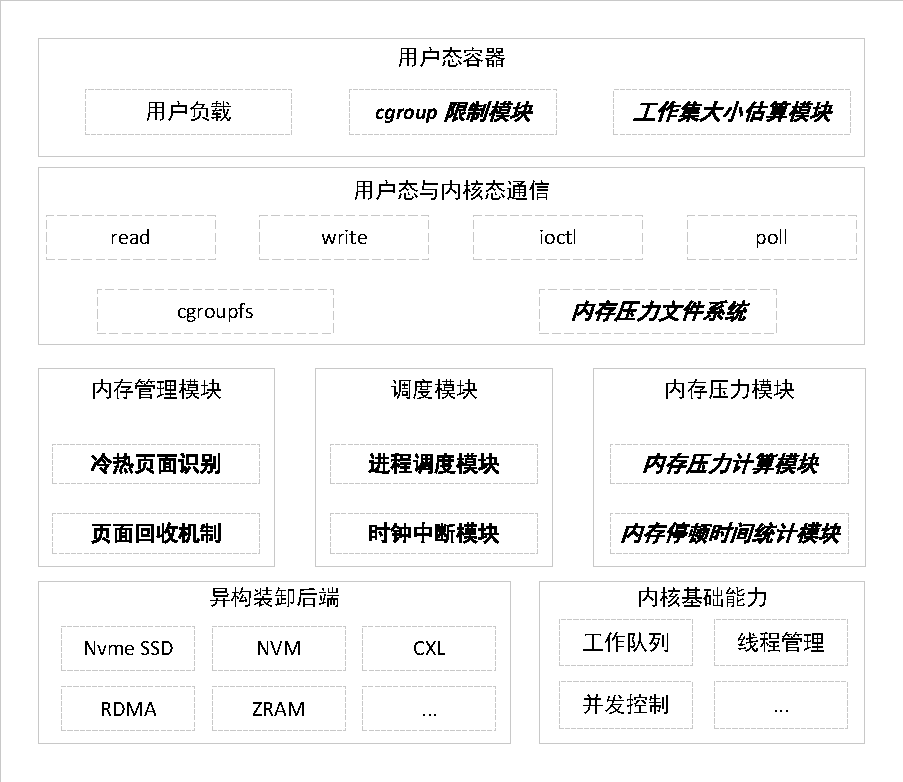
\includegraphics[width=\textwidth,keepaspectratio]{架构层次图.pdf}
    \caption{架构层次图}
    \label{fig:system_architecture_hierarchy}
\end{figure}

\section{需求分析与设计目标}

本方案旨在为异构后端提供一个基于内存压力的自适应透明卸载的框架,用户只需要基于异构卸载后端实现基于 Frontswap 接口,接入 swap 后端中,就可以实现冷页面的主动卸载。该框架具有显著的通用性和可扩展性,无需针对不同的用户负载特征和异构后端存储进行专门适配。


具体而言,本系统的设计目标涵盖以下功能性需求:
\begin{itemize}
\item 框架应该在同一负载下,针对不同的异构卸载后端,产生不同的内存压力。
\item 框架应该根据内存压力,自适应的调整工作集大小,实现冷页面的主动卸载。
\item 框架应该正确的调节\(swappiness\)参数,优化文件密集型应用。
\item 框架应实现冷页面的透明卸载,且无需修改应用程序代码。
\item 框架应确保用户负载的执行性能不受影响。
\end{itemize}

在非功能性需求方面,主要包括以下要点:
\begin{itemize}
\item 框架应采用非侵入式设计,鉴于涉及内核操作,需充分考虑内核稳定性
\item 框架应尽可能降低自身开销,以避免对用户负载的执行性能产生负面影响
\end{itemize}

\section{系统架构}
本论文提出的面向异构后端的自适应主动卸载架构如图 \ref{fig:system_architecture_hierarchy} 所示。该架构采用内核态-用户态协同设计模式,旨在实现对容器内存压力的精确感知与主动卸载。图中加粗斜线表示新增模块,加粗部分表示修改模块。

框架底层由异构卸载后端和内核基础能力构成。异构卸载后端支持多种卸载后端,包括NVMe SSD、NVM、CXL、RDMA和ZRAM等,可通过实现 Frontswap 接口来接入 swap 以实现内存卸载。内核基础能力为框架运行提供必要支持,涵盖工作队列、线程管理及并发控制等核心功能。

框架的核心组件为内核态模块,由三个主要子模块构成:内存管理模块、调度模块和内存压力模块。内存管理模块包含冷热页面识别与页面分配功能,其中冷热页面识别与页面分配模块进行了改动;调度模块由进程调度与时钟中断模块组成,在每次调度时更新内存停顿时间统计模块中的累计时间;内存压力模块由内存压力计算与内存停顿时间统计模块组成,均为新增模块。

用户态容器包含三个核心模块:用户负载、 CGroup 限制模块及工作集大小估算模块。用户负载代表容器内运行的实际应用程序; CGroup 限制模块基于Linux内核的 CGroup 机制,对容器内存资源使用进行约束;工作集大小估算模块根据内核态提供的内存压力信息,动态估算容器工作集大小,并据此调整 CGroup 内存限制,实现内存的主动卸载。

用户态与内核态之间通过多种通信机制实现交互。 CGroupsfs 用于和内核态的 CGroup 模块交互,获取和设置 CGroup 的内存限制。此外,通过自定义的内存压力文件系统(Memory Pressure File System, mpfs)接口获取内核态内存压力信息,并对容器内存资源配置进行动态调整。

\subsection{内存压力模块}

内存压力模块作为本架构的核心组件,承担着将内核检测到的内存短缺状况进行量化的关键任务,为用户态的工作集估计算法提供数据支撑,实现冷页面的主动卸载。

内存压力模块的核心组件为内存停顿时间统计单元。该单元通过在内核同步内存回收路径上实施精细化插桩,捕获因内存分配请求无法立即满足而触发的同步回收事件。对于每个同步回收事件,系统在其开始和结束时更改状态,计算累计时间。在每次时钟中断和调度发生时,通过状态判断更新累计时间。

内存压力计算单元基于内存停顿时间统计单元提供的原始数据,采用加权平均、指数平滑等统计方法进行分析。该单元不仅考虑最近一次停顿时间,还综合历史数据,生成能够平滑反映内存压力变化的量化指标。该指标设计旨在平衡响应速度与稳定性,既能够及时捕捉内存压力突变,又可避免因短期波动导致的误判,从而为用户态提供可靠的决策依据。具体细节将在第\ref{sec:基于同步内存回收延迟的内存压力量化算法}节介绍。


\subsection{内存管理模块}

内存管理模块作为Linux内核的核心组件,负责系统物理内存的分配、回收与管理。本框架主要修改了冷热页面识别机制和内存回收机制的部分代码。

冷热页面识别机制是内存回收和页面置换策略的基础。正确识别冷热页面才能在不损失性能的前提下,实现冷页面的主动卸载。本研究主要针对回收页面中匿名页和文件页的识别比例做了优化,通过算法得到文件页的重用距离判断该文件页是否发生了频繁的换入换出,自适应的调节匿名页和文件页的回收比例。具体细节将在第\ref{sec:基于重用距离的冷热页面优化}节介绍。

此外,为支持内存压力模块的统计需求,本框架在内存分配与回收的关键路径上实施了插桩,用于收集分配延迟、回收延迟等详细内存操作信息,为系统性能分析与优化提供了数据支撑。


\subsection{通信模块}

通信模块负责实现内核态与用户态之间的高效数据交互,确保内存压力指标能够实时、准确地传递至用户态的容器管理组件。本模块基于 proc 虚拟文件系统实现了 mpfs ,通过创建特定入口以标准文件I/O操作方式暴露内存压力信息。该入口采用百分比形式呈现内存压力指标,用户态程序可通过 read 系统调用直接获取相关信息。

为支持用户态程序对内存压力变化的实时响应,通信模块实现了 poll 系统调用接口。该接口采用事件驱动模型,允许用户态程序注册对特定文件描述符的事件监听。当内存压力指标超过预设阈值时,内核通过 poll 机制主动通知用户态程序,有效避免了频繁轮询带来的性能开销。这种事件驱动设计显著提升了用户态程序响应内存压力变化的及时性与效率。具体细节将在第\ref{sec:mpfs_implementation}节介绍。

\subsection{用户态容器}

用户态容器作为应用程序运行的隔离环境,是本架构实现内存压力感知与动态资源调整的执行单元。容器架构包含以下核心组件:

用户负载组件代表容器内运行的实际应用程序或服务。这些应用程序对底层的内存压力感知与资源调整机制保持透明,无需任何修改即可受益于架构提供的性能优化。

工作集大小估算模块是容器的关键组件,负责基于通信模块提供的内存压力信息,动态评估容器的当前工作集大小,确定主动卸载内存的规模。该模块基于非线性反馈控制原理,在检测到高内存压力时扩展内存配置,在低压力状态下则主动收缩内存分配,实现精确的工作集动态调整,从而实现冷页面的主动卸载。

 CGroup 限制模块利用Linux内核的 CGroup 机制,对容器的内存资源使用实施动态约束。该模块通过与 CGroupsfs 文件系统交互,实时调整容器的软限制参数。工作集大小估算模块的输出作为 CGroup 限制模块的核心输入,指导其设置合理的内存限制,实现冷页面的主动卸载。具体细节将在第\ref{sec:pressure_based_model}节介绍。

\section{运行流程}

本节介绍系统运行流程,从框架初始化以及用户态和内核态的交互流程来介绍内存压力模块以及用户态容器组成的完整系统的典型流程,以进一步说明各个模块的之间的关系。

\subsection{框架初始化}

\begin{figure}[htb]
    \centering
    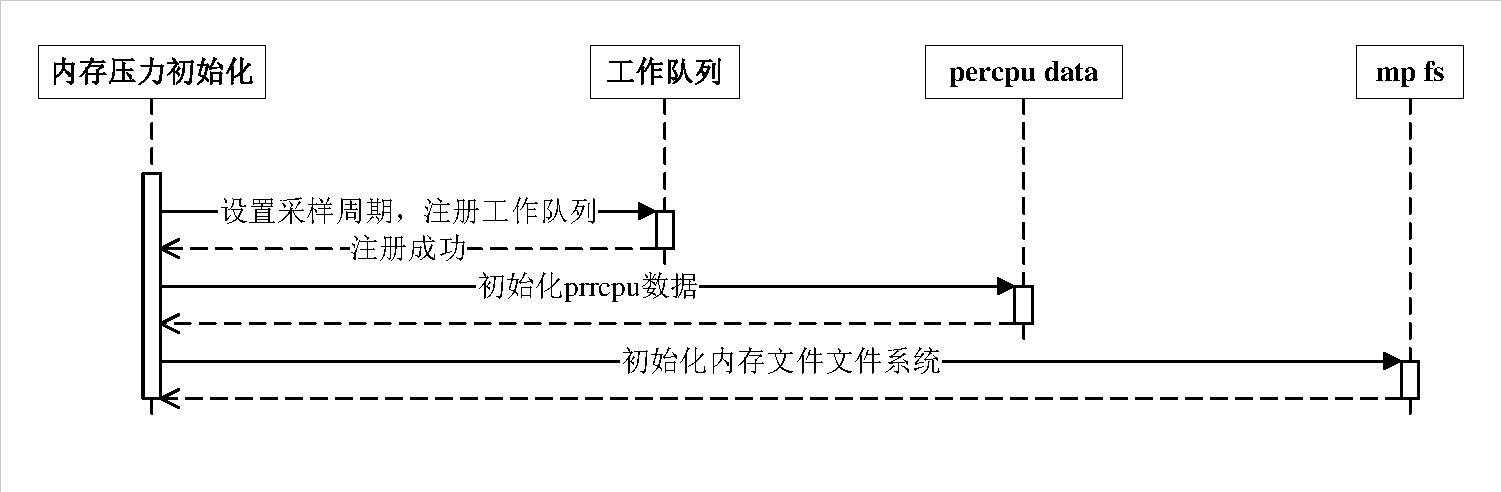
\includegraphics[width=\textwidth,keepaspectratio]{mp初始化.pdf}
    \caption{框架初始化}
    \label{fig:framework_initialization}
\end{figure}

本架构的初始化流程如图 \ref{fig:framework_initialization} 所示,主要包含三个关键阶段:

第一阶段完成采样周期与工作队列的配置。系统通过内核配置设定默认采样周期,并创建专用工作队列。采样周期直接影响内存压力模块的灵敏度,过长会错过瞬时尖峰,过短则增加性能开销。工作队列机制用于异步执行内存压力统计、计算及用户态报告等任务。

第二阶段初始化 Per-CPU 变量。这些变量存储每个 CPU 核心的内存压力统计信息,包括停顿累计时间、非空闲时间等信息。

第三阶段初始化并挂载 mpfs 文件系统。该虚拟文件系统通过内核 mount 调用挂载于指定目录,并与 VFS 层集成。mpfs 通过标准文件操作将内存压力信息暴露给用户态,使应用程序能够实时监控和响应系统内存状态。

\subsection{面向异构后端的自适应主动卸载框架的执行流程}
\label{sec:面向异构后端的自适应主动卸载框架的执行流程}

\begin{figure}[htb]
\centering
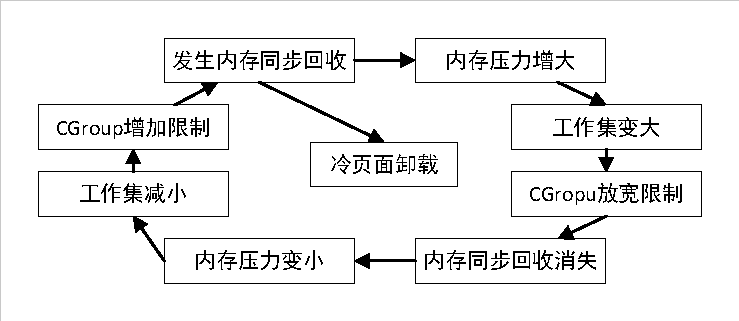
\includegraphics[width=\textwidth,keepaspectratio]{负反馈.pdf}
\caption{负反馈闭环执行流程}
\label{fig:feedback_loop}
\end{figure}

\begin{figure}[htb]
\centering
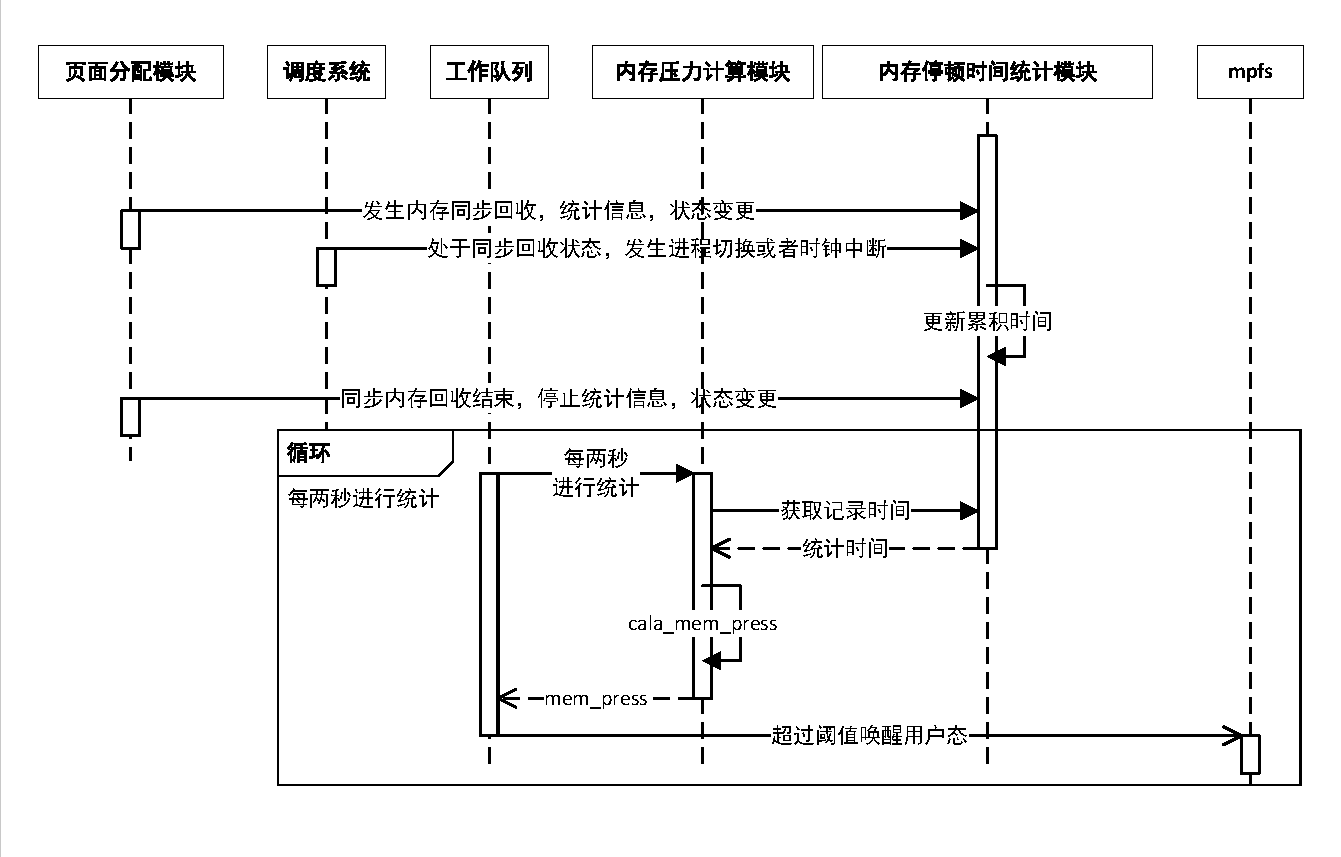
\includegraphics[width=\textwidth,keepaspectratio]{序列图1.pdf}
\caption{执行流程1}
\label{fig:kernel_sequence_diagram_1}
\end{figure}

\begin{figure}[htb]
\centering
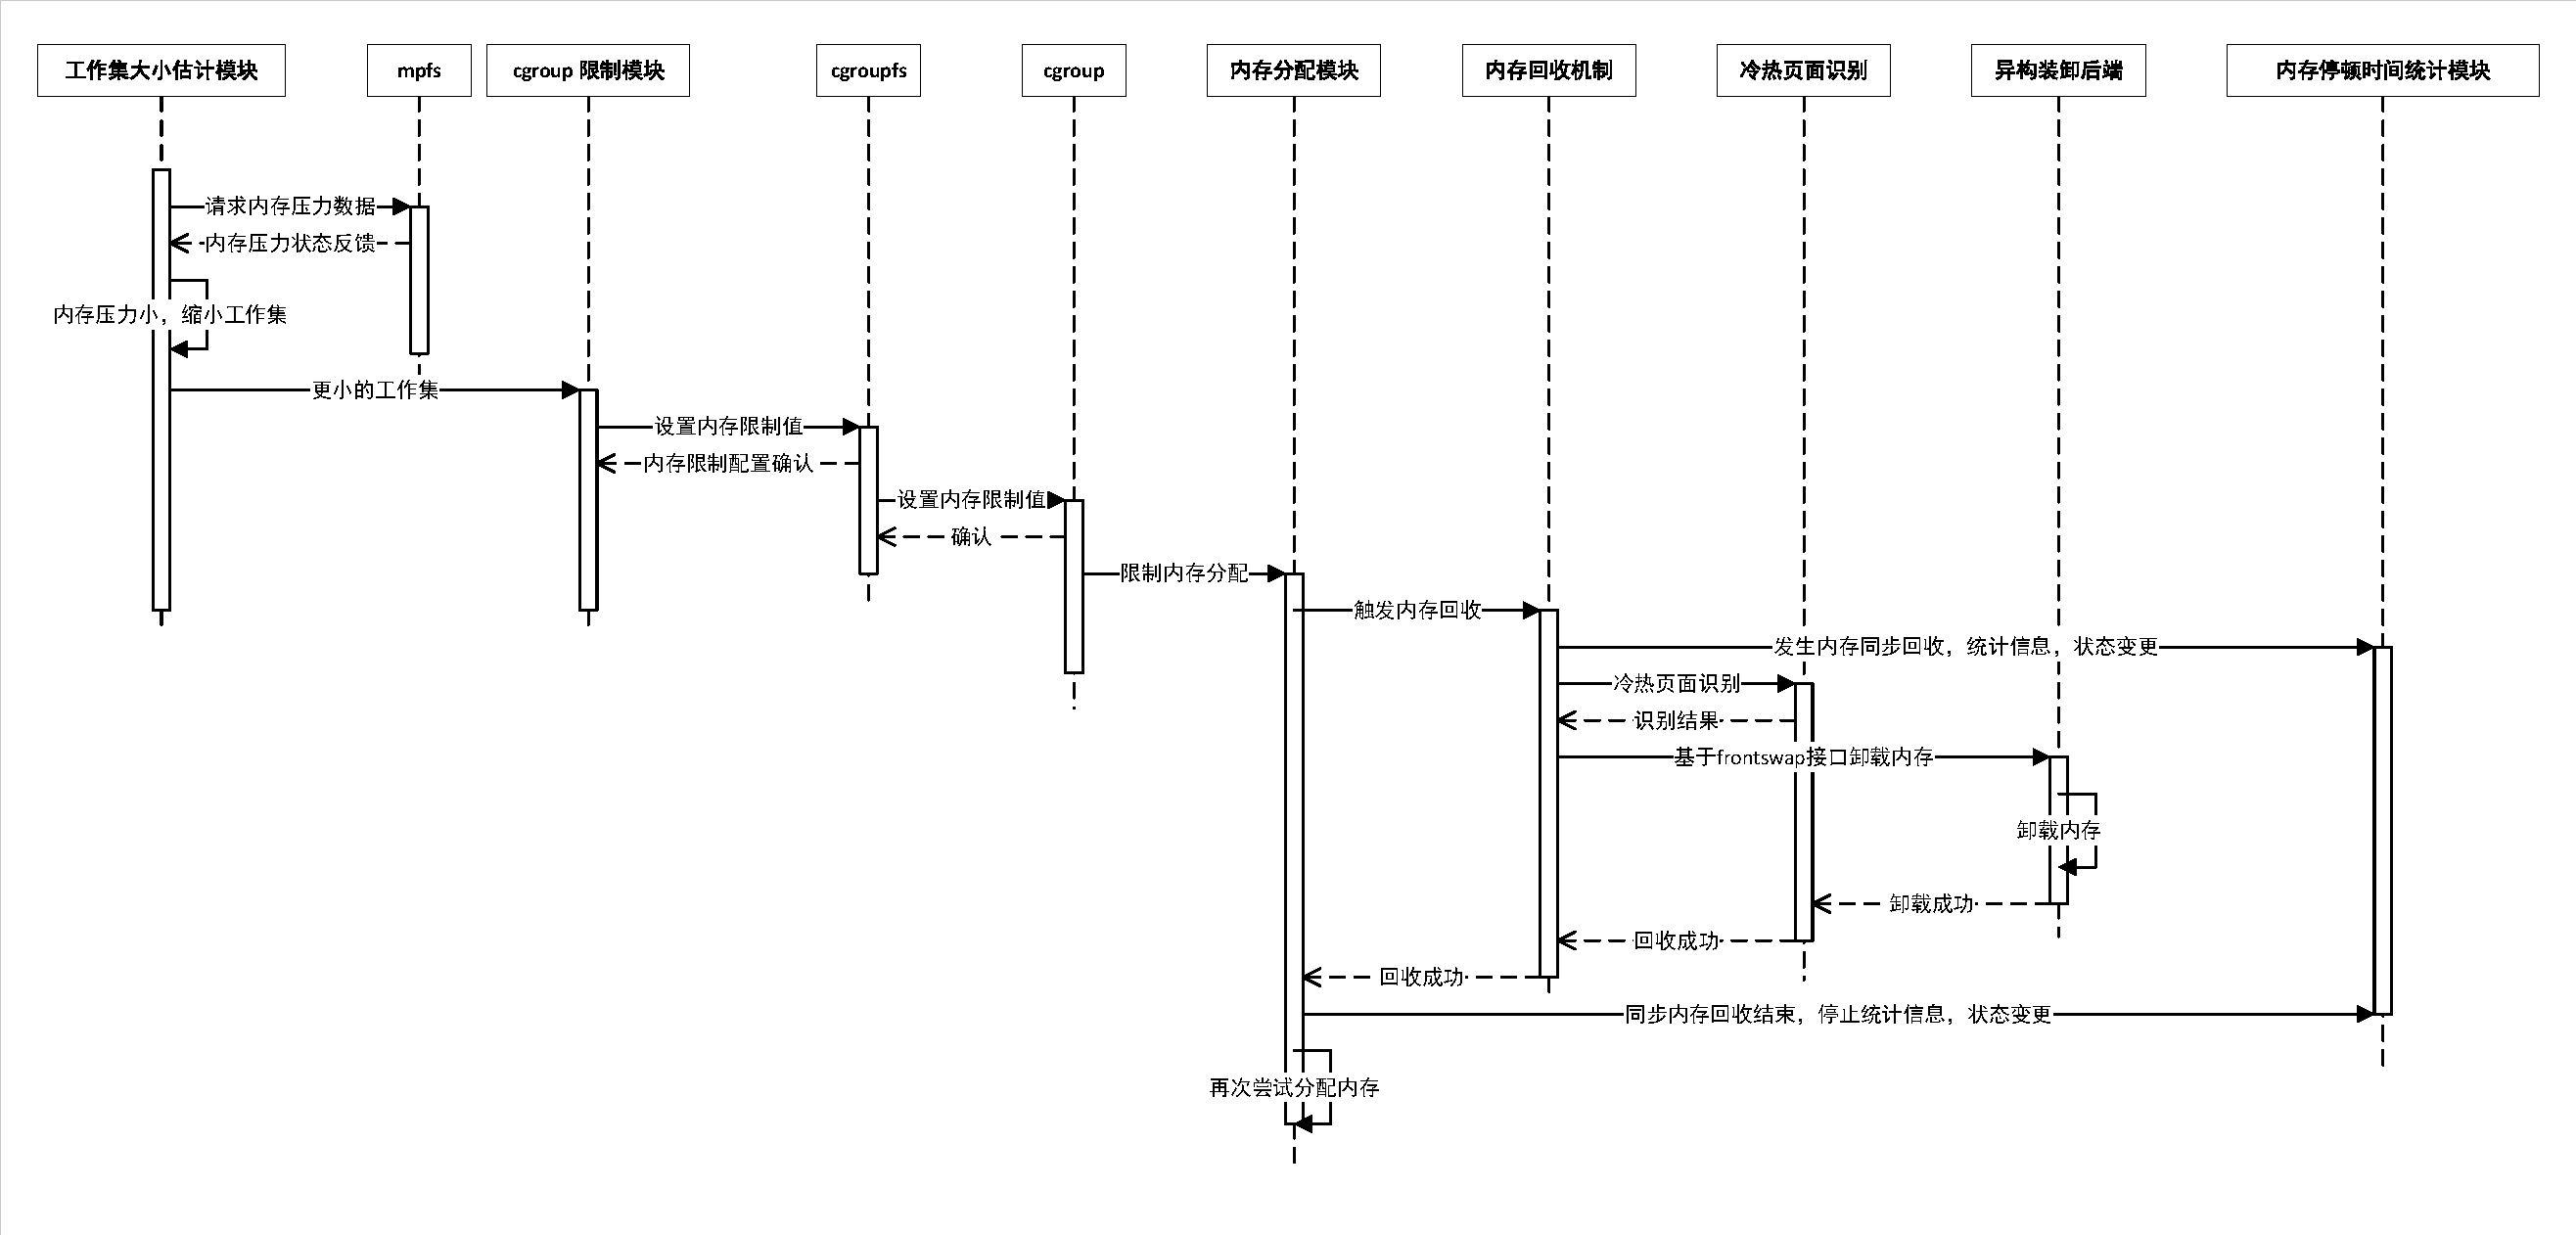
\includegraphics[width=\textwidth,keepaspectratio]{序列图2.pdf}
\caption{执行流程2}
\label{fig:kernel_sequence_diagram_2}
\end{figure}

\begin{figure}[htb]
\centering
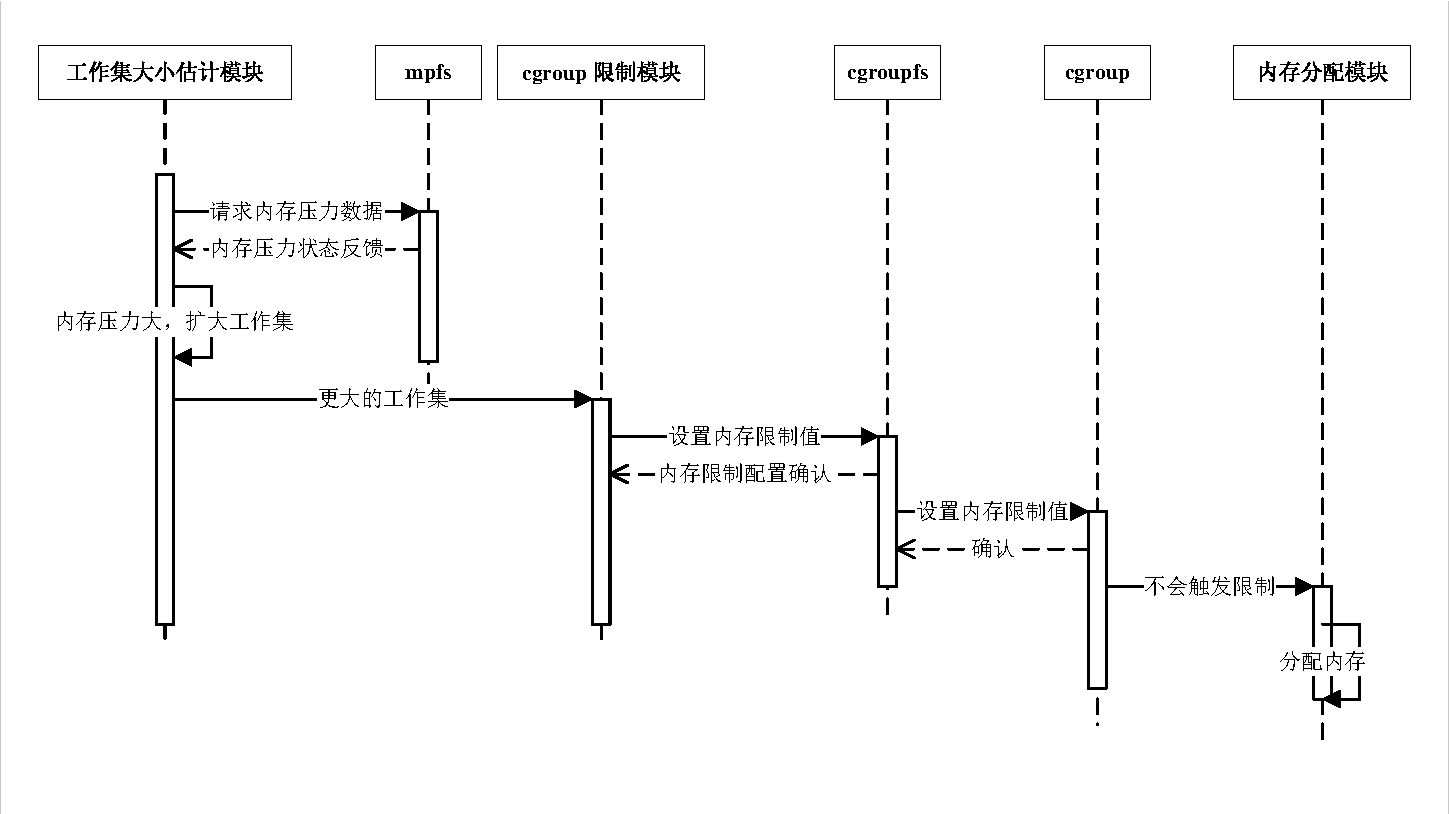
\includegraphics[width=\textwidth,keepaspectratio]{序列图3.pdf}
\caption{执行流程3}
\label{fig:kernel_sequence_diagram_3}
\end{figure}

本节详细阐述了框架主动卸载冷页面的机制。该框架通过动态调整工作集大小来响应内存压力变化,工作集大小的调整又反作用于内存压力。在此过程中,通过在第\ref{sec:Linux内存回收机制}节介绍的内存回收机制,将冷页面从物理内存中卸载到异构后端,实现冷页面的主动卸载。整个负反馈过程如图 \ref{fig:feedback_loop} 所示。

基于图 \ref{fig:kernel_sequence_diagram_1}、图 \ref{fig:kernel_sequence_diagram_2} 和图 \ref{fig:kernel_sequence_diagram_3},本研究详细阐述了面向异构后端的自适应主动卸载框架的执行流程及各模块间的交互机制:

\textbf{阶段一:内存压力监测}:图 \ref{fig:kernel_sequence_diagram_1} 展示了内存压力监测阶段。该阶段始于内存分配请求的发起。当系统无法立即满足应用程序的内存请求时,触发内存同步回收机制。内存停顿时间统计模块介入,记录系统状态并启动回收过程的持续跟踪。在回收过程中,系统发生进程切换或时钟中断时,检查状态并更新累计时间,为后续内存压力分析提供数据支持。同步回收结束时,统计模块停止记录并完成状态变更。内存压力计算模块以采样周期进行一次周期性统计,采用加权平均、滑动窗口等统计方法处理原始数据,生成量化的内存压力指标。若注册了 poll 且超过阈值,则唤醒用户态。

\textbf{阶段二:内存压力小,工作集调整与冷页卸载}:图 \ref{fig:kernel_sequence_diagram_2} 展示了内存压力较小时的处理流程。用户态的工作集大小估计模块通过 mpfs 接口发起内存压力数据请求,通常为阻塞式读取操作。内核态的内存压力模块通过 mpfs 接口反馈最新内存压力状态后,工作集大小估计模块运行特定估计算法。若内存压力较小,则计算出更小的工作集。通过  CGroup  限制模块,将内存限制传递给内核中的  CGroup  机制。 CGroup  机制限制内存分配模块,在后续内存分配时触发内存回收,进而激活内核的内存回收机制,进入内存停顿时间统计模块,开始统计信息并变更状态。同时启动冷热页面识别过程,区分内存中的热页和冷页。冷热页面识别模块完成页面属性识别后,将识别结果告知内存回收机制。系统根据识别结果,利用 Frontswap 接口将冷页从物理内存卸载到预先配置的异构后端中。当冷页成功卸载后,Frontswap 接口向内存回收机制发送卸载成功的反馈信息,停止统计信息并变更状态。

\textbf{阶段三:内存压力大,内存回收与卸载}:图 \ref{fig:kernel_sequence_diagram_3} 展示了内存压力较大时的处理流程。由于发生了同步回收,内存压力增大,工作集大小估计模块计算出更大的工作集,并通过  CGroupfs  调整内存限制。若无内存限制,则不会触发同步回收,内存压力减小后返回第二阶段。

\section{本章小结}

\begin{figure}[htb]
    \centering
    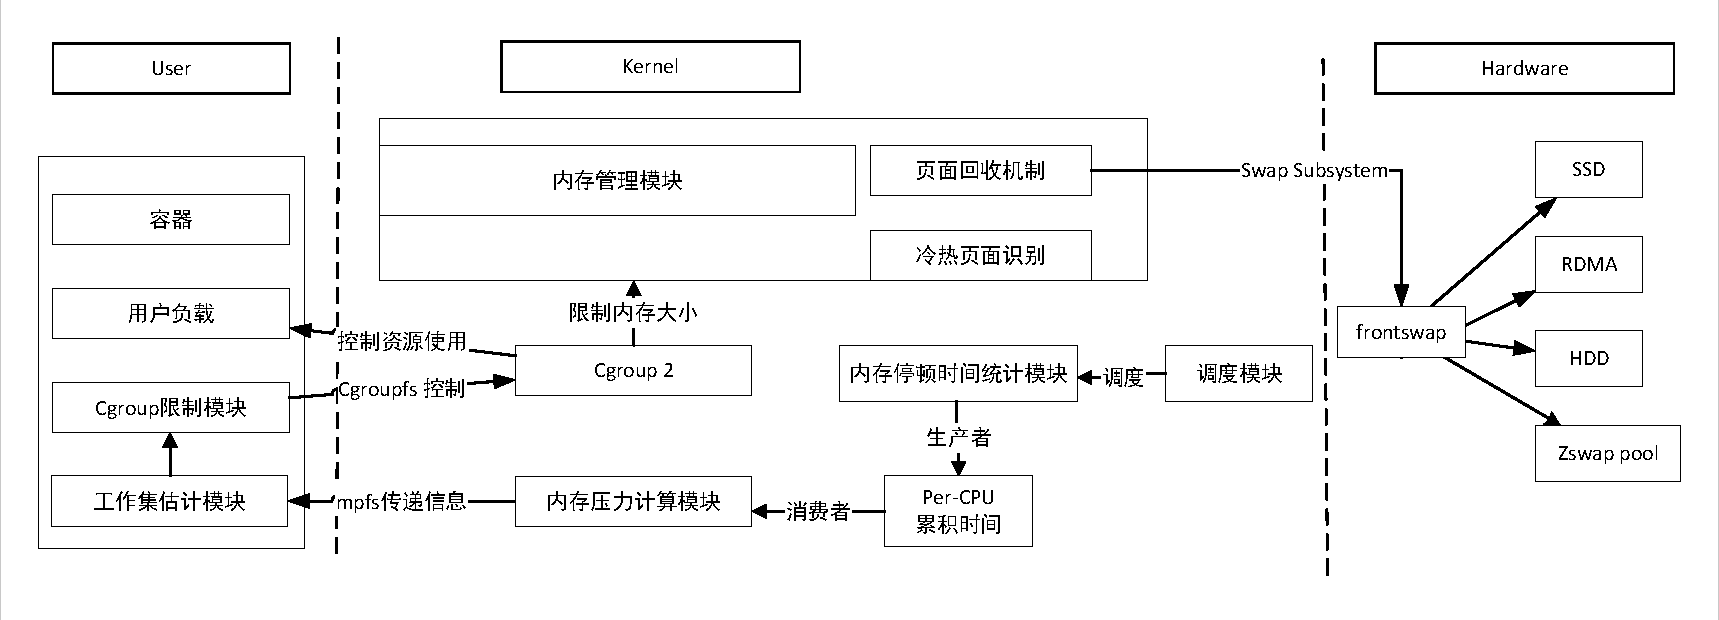
\includegraphics[width=\textwidth,keepaspectratio]{架构图.pdf}
    \caption{系统整体架构}
    \label{fig:system_architecture}
\end{figure}

本章阐述了面向异构后端的自适应主动卸载框架的整体架构及其关键模块,详细介绍了框架初始化流程以及用户态与内核态协同的异构内存资源动态管理机制。系统架构如图 \ref{fig:system_architecture} 所示。

在用户空间层面,系统部署了工作集估算器和 CGroup 管理器两个核心组件。工作集估算器通过 mpfs 持续获取内核态的内存压力信息,并支持基于事件的通知机制以提升响应时效性。 CGroup 管理器负责执行工作集估算器的决策,通过调整 CGroup V2 内存限制参数实现对容器内存资源的动态调控。

内核空间的核心组件为内存压力模块,该模块深度嵌入内核内存管理子系统。内存压力模块采用静态插桩技术,在同步内存回收时记录中断时间片,并与调度系统交互计算回收延迟,生成量化压力信号。该信号通过 mpfs 文件系统周期性暴露给用户空间,同时实现基于事件的通知机制,当内存压力超过预设阈值时主动通知工作集估算器。

系统采用负反馈调节机制实现内存资源的精细化管理。当内存压力较低时,工作集估算器指示 CGroup 管理器收缩容器内存分配上限,主动触发内核页面回收机制,将不活跃页面卸载到后端,实现预先释放,主动卸载策略。当内存压力升高时,内存压力模块迅速检测并更新压力信号,工作集估算器触发负反馈调节,重新评估容器内存需求,计算更大工作集大小, CGroup  管理器通过调整 memory.high 等参数放宽容器内存使用限制,减少缺页中断,保障应用性能。

该机制形成了完整的负反馈闭环:内存压力模块提供实时压力反馈,工作集估算器进行决策, CGroup 管理器执行资源控制,容器工作负载在调整后的资源约束下运行,其内存访问行为进一步影响内核内存压力,实现持续的自适应动态调节。这种协同机制使系统能够灵敏、准确地响应内存压力变化,在保证关键应用性能的同时最大化异构内存系统利用率,有效避免内存过度分配导致的系统抖动和性能下降。
